%!TEX root = ../vernier.tex
\section{Colormap} \label{sec:colormap}
Colormaps are mapping functions that for every point of the domain of interest, assign to it a color based on the scalar value at that point. In this tool, three different color mapping schemes based on the ColorBrewer's \cite{ref:colorbrewer} samples were implemented. A sequential colormap was used to display the current normalized value of a chosen metric, a diverging colormap was used to show the increase/decrease of a given metric from revision $T_{n-1}$ to $T_{n}$, and a categorical colormap was used to group classes from the same package into a single color.

\begin{figure}[H]
	\centering
	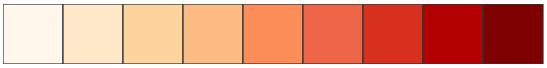
\includegraphics[width=0.6\textwidth]{figures/seq.png}
	\caption{Sequential Colormap}
	\label{fig:seq}
\end{figure}

\begin{figure}[H]
	\centering
	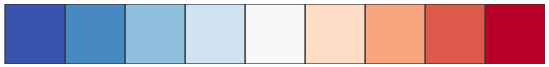
\includegraphics[width=0.6\textwidth]{figures/div.png}
	\caption{Diverging Colormap}
	\label{fig:div}
\end{figure}

\begin{figure}[H]
	\centering
	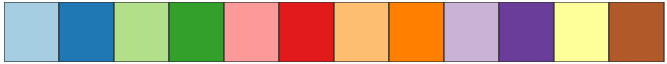
\includegraphics[width=0.6\textwidth,height=1.0cm]{figures/quali.png}
	\caption{Qualitative Colormap}
	\label{fig:quali}
\end{figure}

Combining colormaps with the hierarchical display techniques, we can start to understand more complex phenomena. On figure \ref{fig:colormap_hier} we have used the Sequential Colormap to encode the same metric that is represented by the area of treemap rectangles (i.e. number of lines of code) in the last collected revision of the ExoPlayer project. Between the two representations there is a color legend that displays the full colormap and presents the minimum and maximum values of the selected metric for the whole project's history. The ring sections that represent packages in the Sunburst Diagram are colored with the recursive average value of its children, allowing for objective comparison between packages, and not only classes.

\begin{figure}[H]
  \centering
  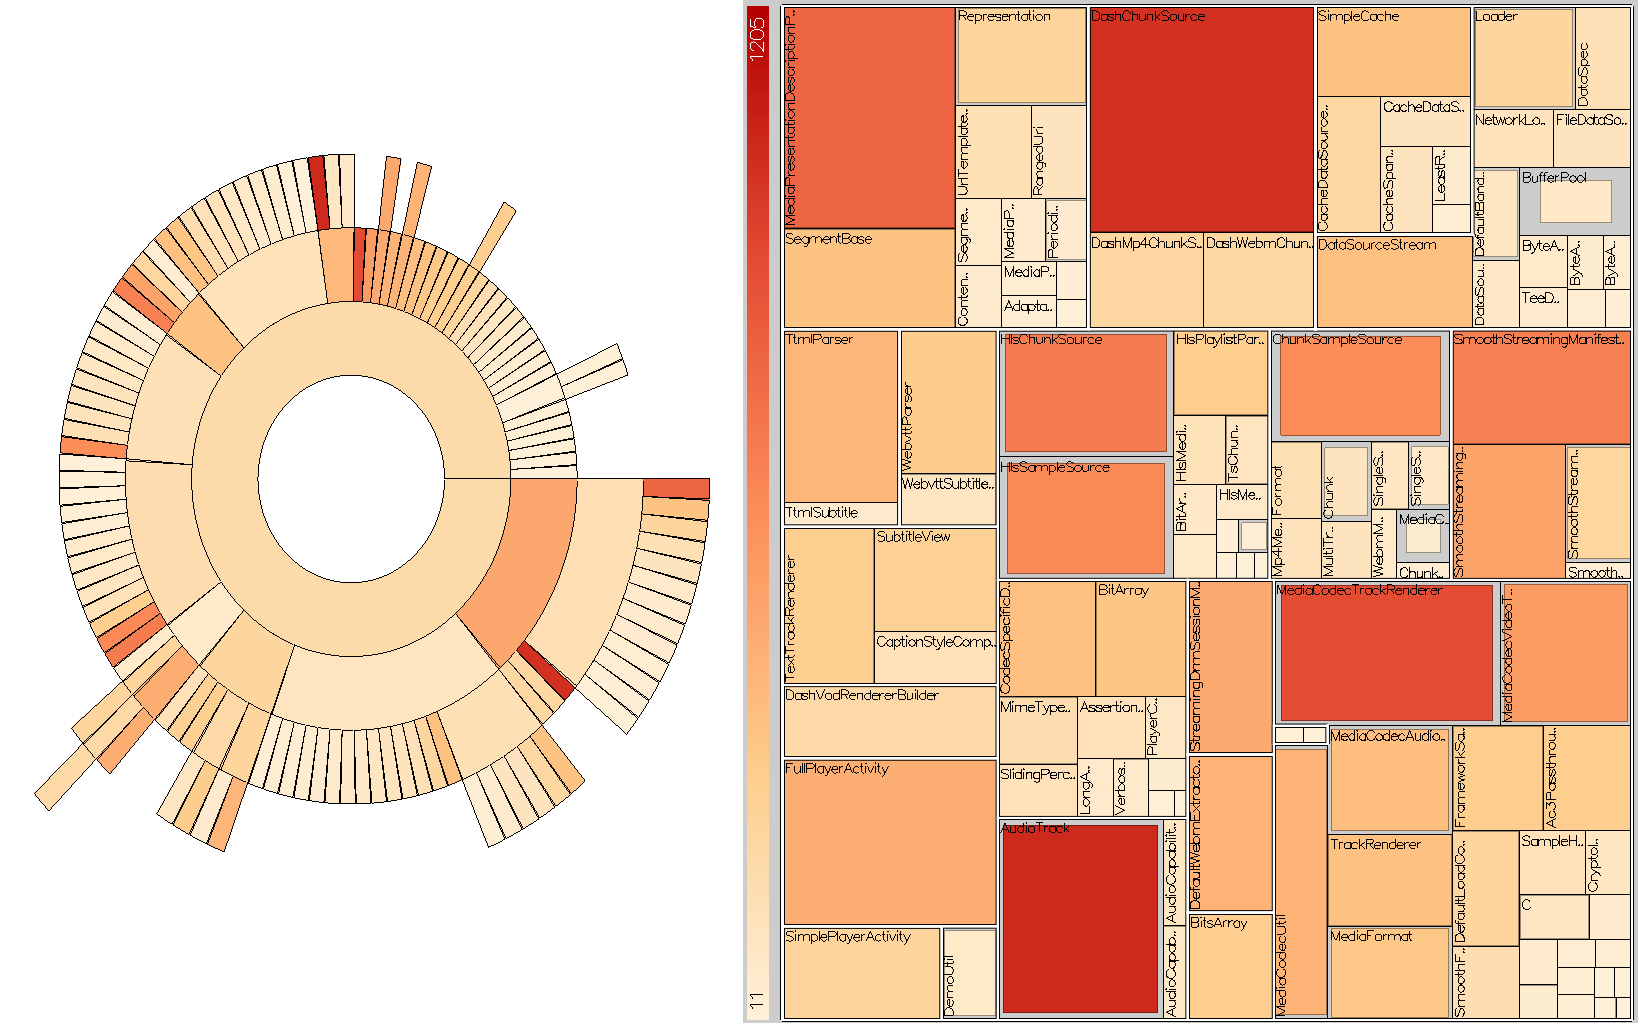
\includegraphics[width=1\textwidth]{figures/colormap_hier.png}
  \caption{}
  \label{fig:colormap_hier}
\end{figure}

The divergent colormap can be used to analyze the activity between revisions. On figure \ref{fig:colormap_div_sun}, we can see that a lot of effort has been put int order to decrease the size of most classes, with exception of the ones in package A, which have increased significantly. This might suggest that refactoring with code movement took place in this revision.

\begin{figure}[H]
  \centering
  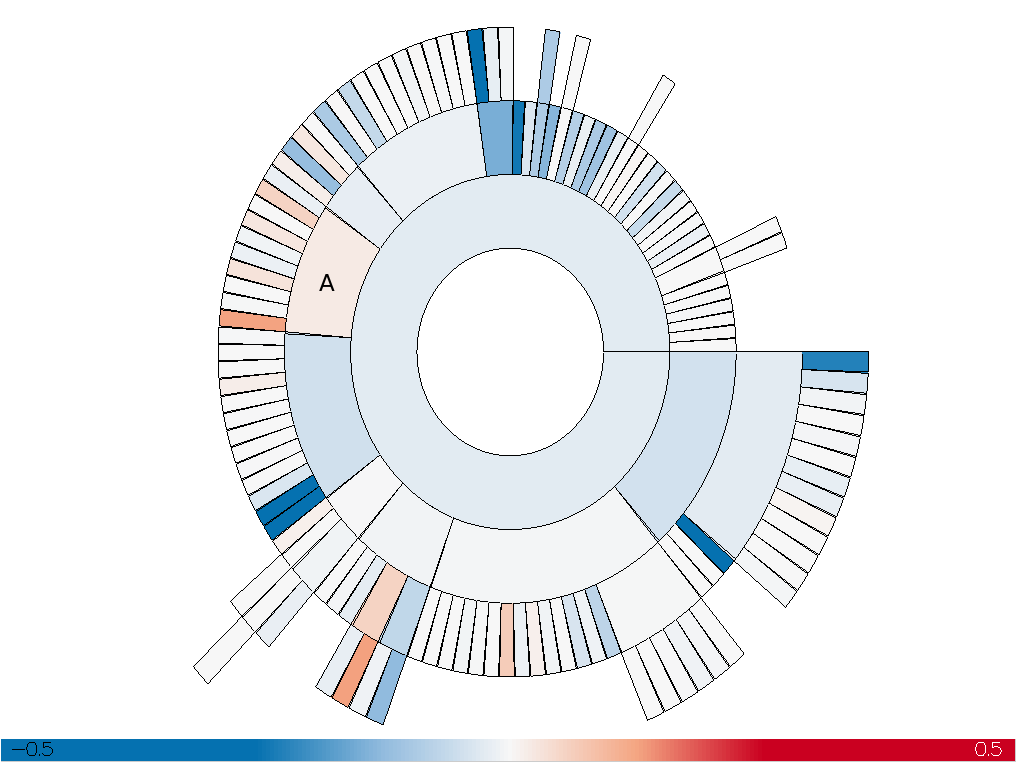
\includegraphics[width=1.0\textwidth]{figures/colormap_div_sun.png}
  \caption{}
  \label{fig:colormap_div_sun}
\end{figure}
